\documentclass[tikz,border=2mm]{standalone}
\usetikzlibrary{positioning,matrix,decorations.pathmorphing,calc}

\definecolor{BorderBlue}{RGB}{33, 51, 148}
\definecolor{CoinColor}{RGB}{245, 230, 61}

\definecolor{InkyColor}{RGB}{0, 165, 236}
\definecolor{ClydeColor}{RGB}{255, 130, 0}
\definecolor{PinkyColor}{RGB}{254, 171, 200}
\definecolor{BlinkyColor}{RGB}{251, 1, 0}

\pgfmathsetseed{\number\pdfrandomseed}

% #1 init
% #2 exit
% #3 coin amount
\def\coins#1#2#3{
  \foreach \x in {1,...,#3}{%
    \pgfmathsetmacro{\current}{\x/#3}%
    \fill[CoinColor] ($(#1)!\current!(#2)$) circle (0.1);
  }
}

\begin{document}
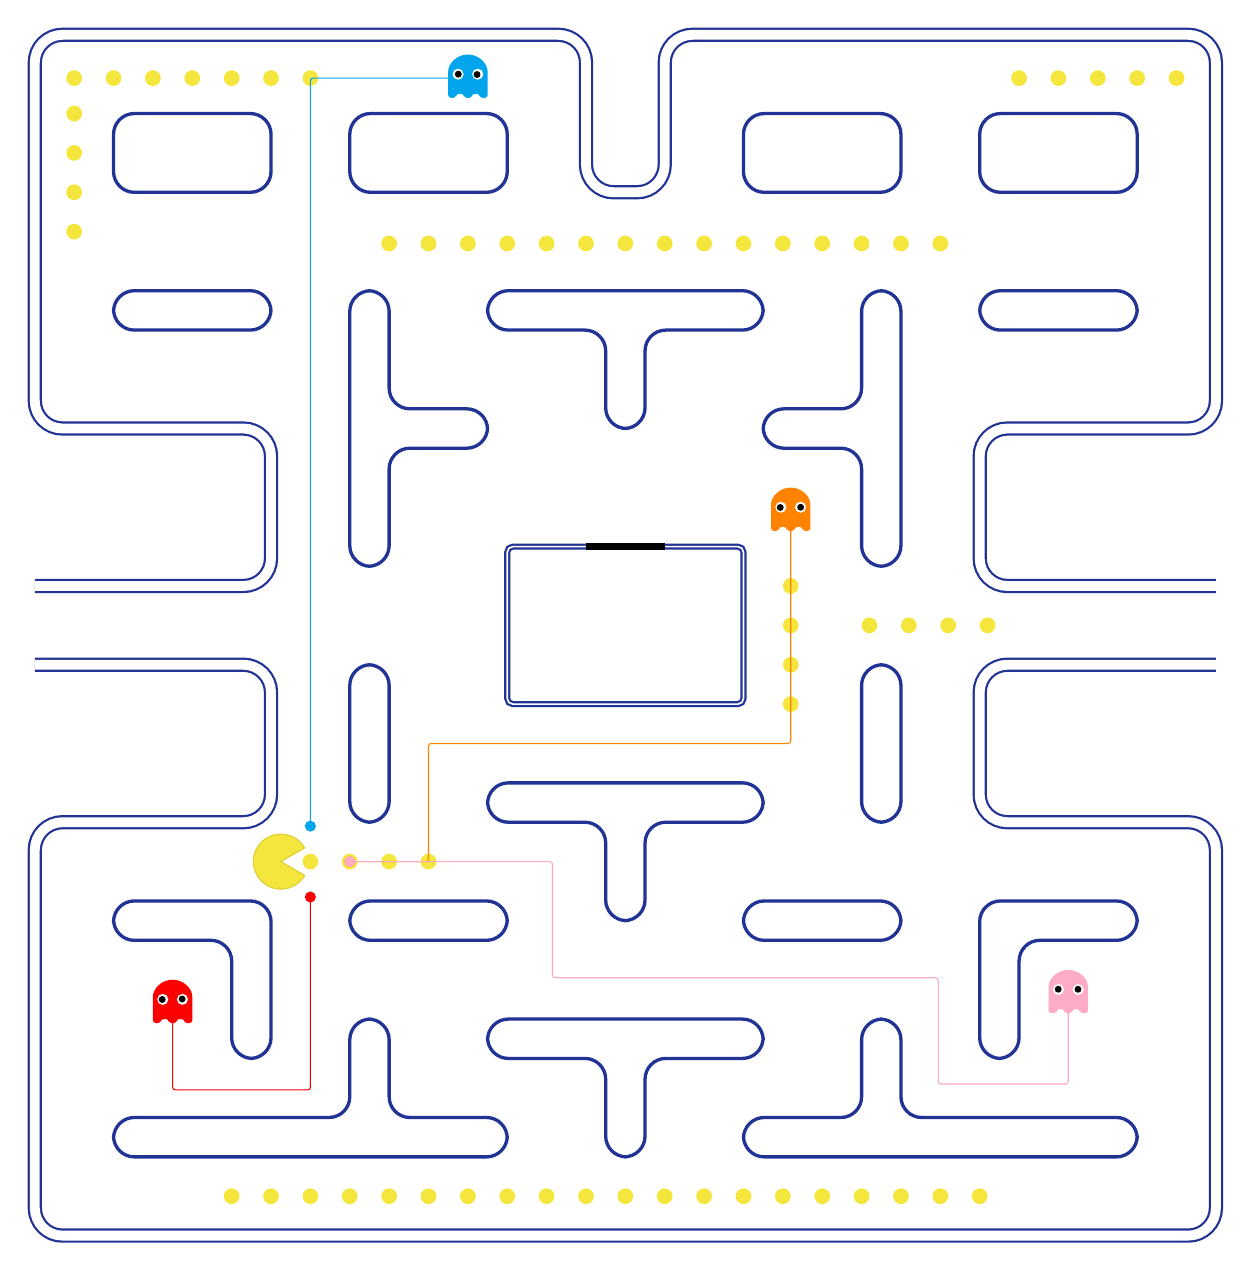
\begin{tikzpicture} [border/.style={double,double distance=0.125cm,BorderBlue,rounded corners=10pt,thick}, block/.style={very thick,BorderBlue,rounded corners=7.5pt}]

\draw[border] (0,-7) -| ++ (3,2) -| ++(-3,5) -| (7,-2) -| ++ (1,2) -| ++ (7,-5) -| ++(-3,-2) -- ++(3,0);
\draw[border] (0,-8) -| ++(3,-2) -| ++(-3,-5.25) -| ++(15,5.25) -| ++(-3,2) -- ++(3,0);

\draw[double,BorderBlue,thick,rounded corners=2pt] (6,-6.5) rectangle ++ (3,-2); \draw[black,line width=2.5pt] (7,-6.5) -- ++(1,0);

% upper left stuff
\draw[block] (1,-1) rectangle ++(2,-1) (4,-1) rectangle ++(2,-1) (1,-3.25) rectangle ++(2,-0.5);
\draw[block] (15-1,-1) rectangle ++(-2,-1) (15-4,-1) rectangle ++(-2,-1) (15-1,-3.25) rectangle ++(-2,-0.5);

% draw the 'T' palisade
\draw[block] (5.75,-3.25) -| ++(3.5,-0.5) -| ++(-1.5,-1.25) -| ++(-0.5,1.25) -- ++(-1.5,0) -- cycle;
\draw[block] (5.75,-9.5) -| ++(3.5,-0.5) -| ++(-1.5,-1.25) -| ++(-0.5,1.25) -- ++(-1.5,0) -- cycle;
\draw[block] (5.75,-12.5) -| ++(3.5,-0.5) -| ++(-1.5,-1.25) -| ++(-0.5,1.25) -- ++(-1.5,0) -- cycle;

% rotated upper left
\draw[block] (4,-3.25) -| ++(0.5,-1.5) -| ++(1.25,-0.5) -| ++(-1.25,-1.5) -- ++(-0.5,0) -- cycle;
% rotated upper right
\draw[block] (15-4,-3.25) -| ++(-0.5,-1.5) -| ++(-1.25,-0.5) -| ++(1.25,-1.5) -- ++(0.5,0) -- cycle;

% left and right blocks
\draw[block] (4,-8) rectangle ++ (0.5,-2) (15-4,-8) rectangle ++ (-0.5,-2);
% below sitting verticals
\draw[block] (4,-11) rectangle ++ (2,-0.5) (15-4,-11) rectangle ++ (-2,-0.5);

%Left and Rigth turned 'L'
\draw[block] (1,-11) -| ++ (2,-2) -| ++(-0.5,1.5) -- ++(-1.5,0) -- cycle;
\draw[block] (15-1,-11) -| ++ (-2,-2) -| ++(0.5,1.5) -- ++(1.5,0) -- cycle;

% the huge creepy somewhat lying T's
\draw[block] (1,-14.25) -| ++ (5,0.5) -| ++(-1.5,1.25) -| ++(-0.5,-1.25) -- ++(-3,0) --  cycle;
\draw[block] (15-1,-14.25) -| ++ (-5,0.5) -| ++(1.5,1.25) -| ++(0.5,-1.25) -- ++(3,0) --  cycle;


% Some Coins upper left
\coins{0,-0.55}{3.5,-0.55}{7};
\coins{0.5,-0.5}{0.5,-2.5}{4};
\coins{4,-2.65}{11.5,-2.65}{15};

\coins{15,-0.55}{15-2.5,-0.55}{5};
\coins{9.6,-6.5}{9.6,-8.5}{4};
\coins{10.1,-7.5}{12.1,-7.5}{4};

\coins{2,-14.75}{12,-14.75}{20};
\coins{3,-10.5}{5,-10.5}{4};


% draw: pacman:
\draw[thin,CoinColor!90!black,fill=CoinColor] (3.125,-10.5) -- ++(30:0.35) arc[radius = 0.35,start angle=30,delta angle=300] -- cycle;

% ghost:
% #1 where #2 color
\def\drawGhost#1#2{
  \fill[#2,rounded corners=1pt] (#1) arc[radius = 0.25,start angle=180,delta angle=-180] -- ++(0,-0.3) -| ++(-0.1,0.05) -| ++(-0.1,-0.05) -| ++(-0.1,0.05) -| ++(-0.1,-0.05) -- ++(-0.1,0) -- cycle;
  % get random offsets for more fun:
  \pgfmathsetmacro{\eyeX}{0.25*rand}\pgfmathsetmacro{\eyeY}{0.15*rand}
  \fill[white] (#1)++(0.25/2,0) circle (2pt); \fill (#1)++(\eyeX pt,\eyeY pt)++(0.25/2,0) circle (1.25pt);
  \pgfmathsetmacro{\eyeX}{0.25*rand}\pgfmathsetmacro{\eyeY}{0.15*rand}
  \fill[white] (#1)++(0.75/2,0) circle (2pt); \fill (#1)++(\eyeX pt,\eyeY pt)++(0.75/2,0) circle (1.25pt);
}
\drawGhost{5.25,-0.5}{InkyColor}
% draw targetpath for the ghost
\draw[InkyColor,thin,rounded corners = 1pt] (5.25,-0.55) -| ++(-1.75,-9.5) node (inkytar) {};\fill[InkyColor] (inkytar) circle (2pt);

\drawGhost{9.35,-6}{ClydeColor}
\draw[ClydeColor,thin,rounded corners = 1pt] (9.35,-6) ++(0.25,0) |- ++(-4.6,-3) |- ++(-1,-1.5) node (clydetar) {};\fill[ClydeColor] (clydetar) circle (2pt);

\drawGhost{12.875,-12.125}{PinkyColor}
\draw[PinkyColor,thin,rounded corners = 1pt] (12.875,-12.125) ++(0.25,0) |- ++(-1.65,-1.2) |- ++(-4.9,1.35) |- ++(-2.575,1.475) node (pinkytar) {};\fill[PinkyColor] (pinkytar) circle (2pt);

\drawGhost{1.5,-12.25}{BlinkyColor}
\draw[BlinkyColor,thin,rounded corners = 1pt] (1.5,-12.25) ++(0.25,0) |- ++(1.75,-1.15) -- ++(0,2.45) node (blinkytar) {};\fill[BlinkyColor] (blinkytar) circle (2pt);

\end{tikzpicture}

\end{document}
